% !TEX root = ../main.tex
%
\chapter{Related Work}
\label{sec:related}

\section{Instant NGP}

Instant Neural Graphics Primitives (Instant NGP) \cite{muller_instant_2022}, developed by NVIDIA, utilizes a multiresolution hash encoding that simplifies models while maintaining high performance and quality.
Its graphical user interface (GUI) plays a crucial role in enhancing accessibility and functionality, making it an important advancement in neural graphics technology.

\cleanparagraph{Simplified User Interaction}
The user interface of Instant NGP facilitates training and visualization of NeRFs \fref{fig:instant-ngp}.
The user is able to interactively explore 3D scenes in real-time and adjust parameters in order to achieve the desired results.

\begin{figure}[h!]
  \centering
  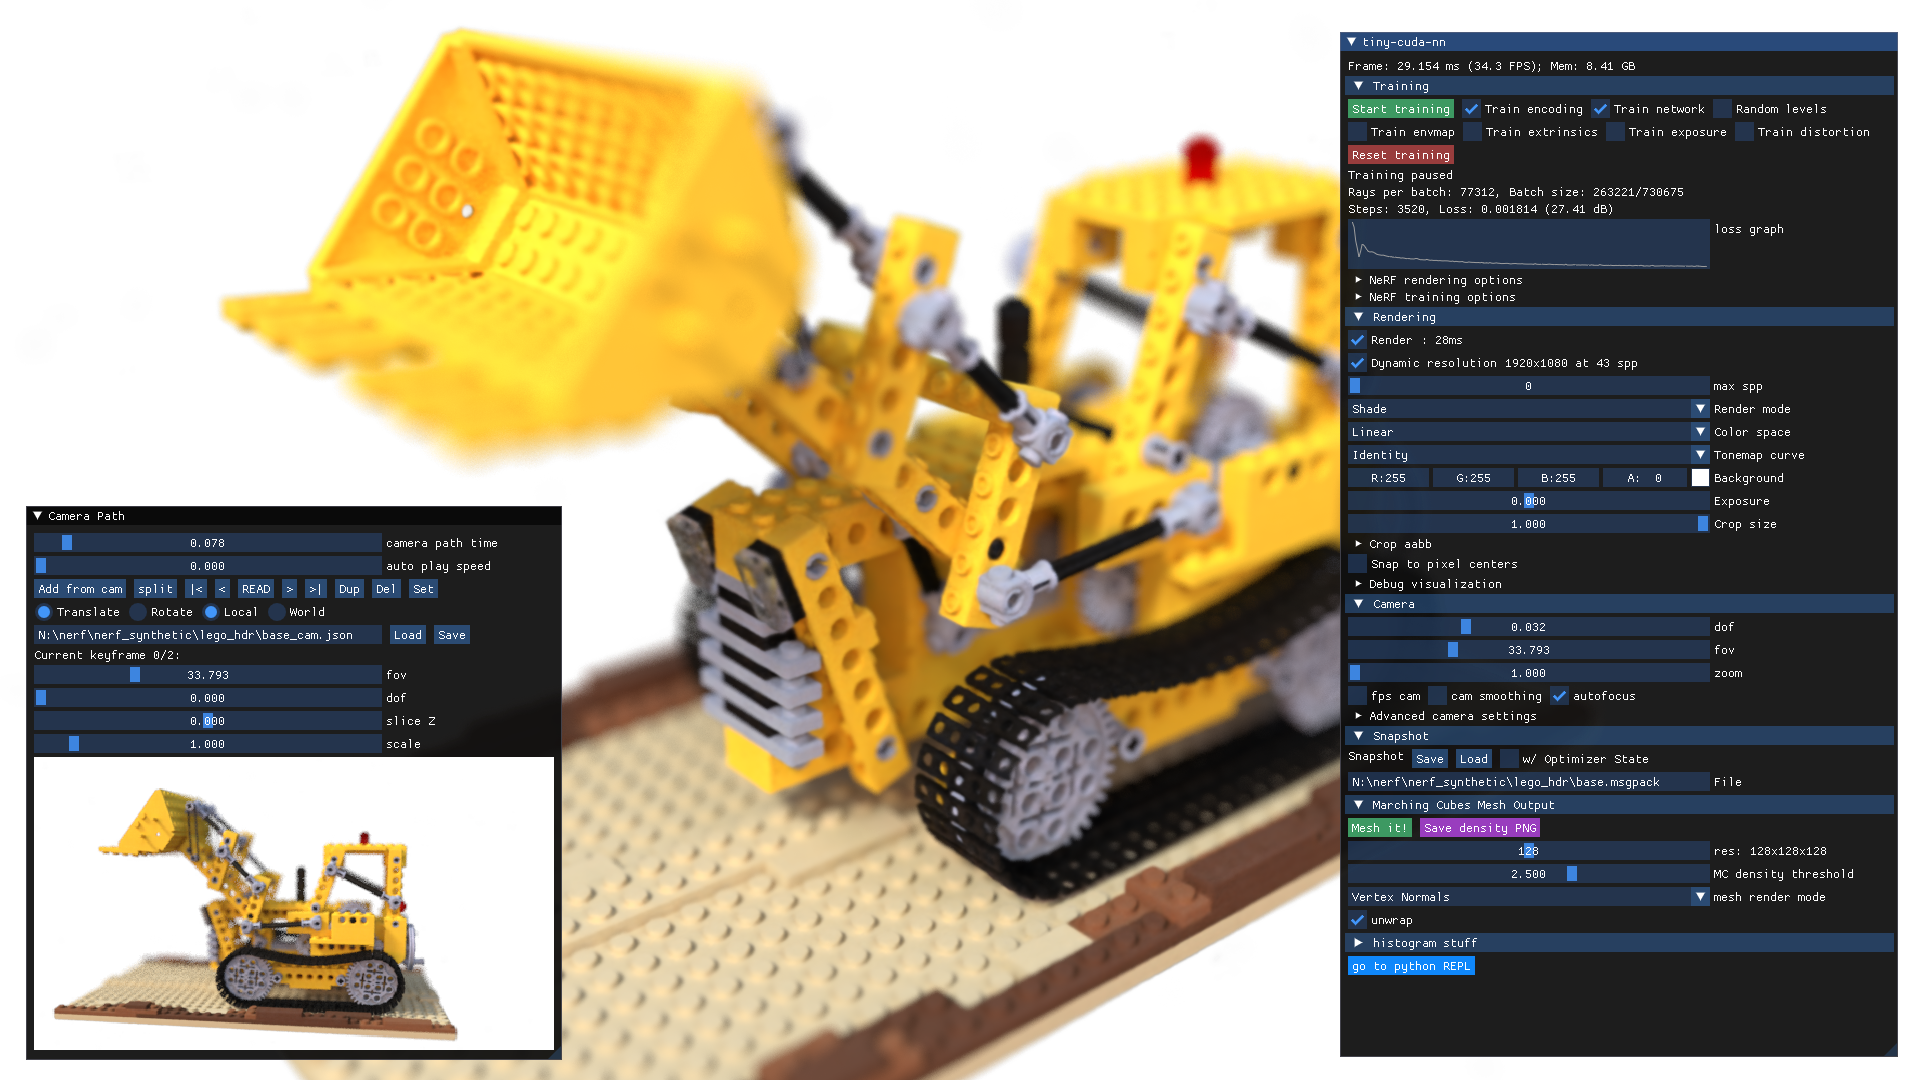
\includegraphics[width=\textwidth]{figures/realted-instant-ngp.png}
  \caption{Instant NGP's GUI rendering a NeRF scene, showing the 3D scene, camera path editor, and training parameters.
   \cite{muller_instant_2022}.}
  \label{fig:instant-ngp}
\end{figure}

\cleanparagraph{VR Mode}
The virtual reality (VR) mode of Instant NGP enhances user interaction by enabling immersive exploration of 3D environments in real-time.
This feature is especially beneficial for professionals like architects and game developers, who can benefit from experiencing their virtual spaces as if they were real.

\cleanparagraph{Camera Path Editor}
Instant NGP's camera path editor allows users to intuitively create and adjust camera trajectories, enhancing the creation of animations.
This tool is essential to professionals in visualization and animation, providing precise control over camera movements for detailed and smooth outputs.

\cleanparagraph{Limitations}
Despite advancements, Instant NGP's technical complexity and reliance on command-line interfaces for key operations remain significant barriers.
These aspects limit its accessibility to those with specific technical skills and deter broader creative applications.
The user experience still requires technical expertise, underscoring the need for more intuitive interfaces that simplify interaction and expand the user base beyond that of technical specialists.

\section{Nerfstudio}
\label{sec:related:nerfstudio}

Nerfstudio \cite{tancik_nerfstudio_2023} represents a significant advance in the accessibility of Neural Radiance Fields to non-technical users.
Its design focuses on modularity, ease of use, and integration capabilities, which are crucial for practical applications and academic research.

\cleanparagraph{Modularity}
Nerfstudio is built on a modular framework that allows users to easily customize and extend their NeRF implementations.
This modularity enables the use of a variety of input data formats, making it versatile for different real-world scenarios and setting it apart from Instant NGP.
A wide range of existing methods are already well integrated into Nerfstudio, including Instant-GPT \cite{muller_instant_2022}, their own Nerfacto \cite{noauthor_nerfacto_nodate} method that combines various existing techniques, and several of the previously mentioned extensions \cite{haque_instruct-nerf2nerf_2023,jan-niklas_dihlmann_signerf_2024}.

\cleanparagraph{Real-Time Web Viewer}
One of the standout features of Nerfstudio is its real-time web viewer, which enables visualization of NeRF training progress and outputs directly through a web browser \fref{fig:nerfstudio-viewer}.
This eliminates the need for high-end local GPU setups, such as in the case of Instant NGP, through remote sessions, broadening the tool's accessibility \cite{noauthor_nerfstudio-projectviser_2024}.

\begin{figure}[h!]
  \centering
  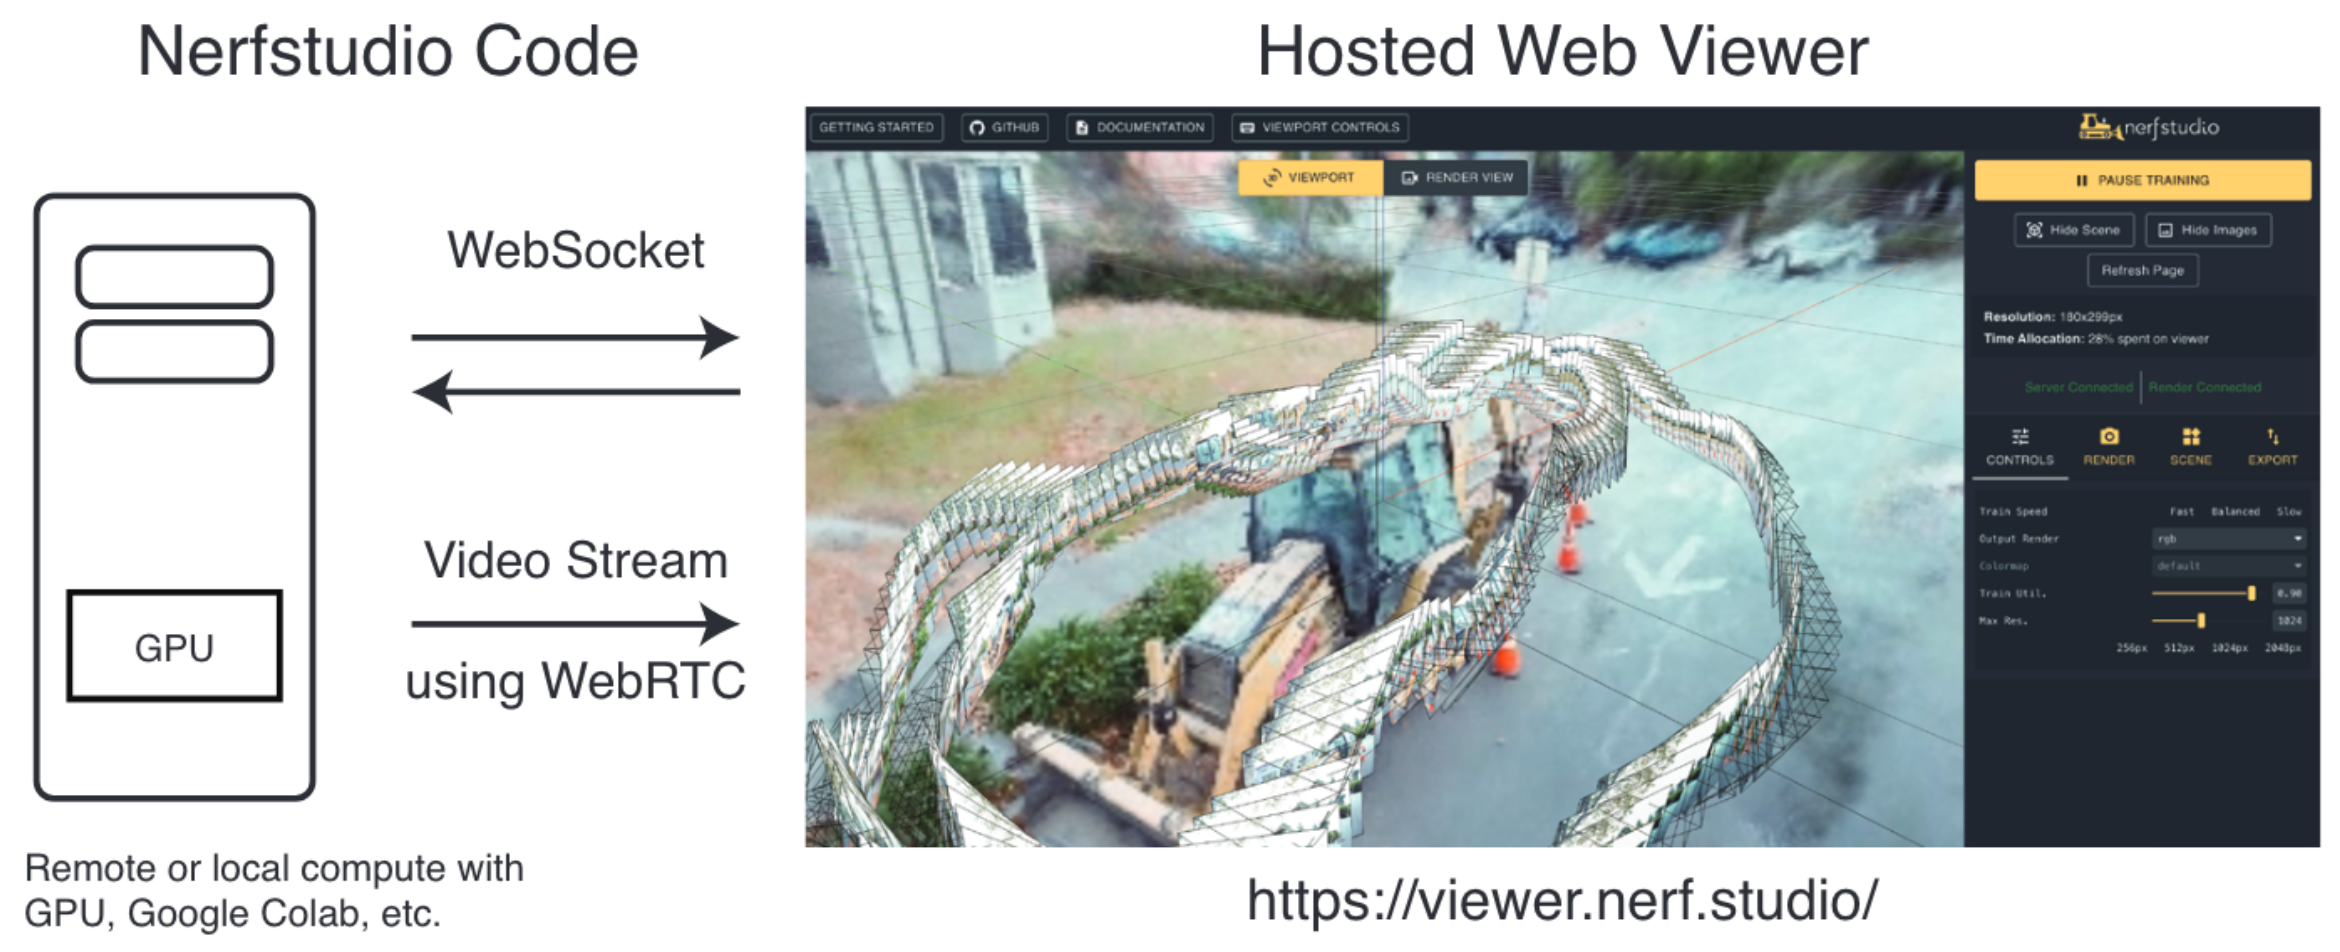
\includegraphics[width=\textwidth]{figures/related-nerfstudio-viewer.png}
  \caption{Nerfstudio's web viewer connected to a remote server running the training \cite{tancik_nerfstudio_2023}.}
  \label{fig:nerfstudio-viewer}
\end{figure}

\cleanparagraph{Flexibility of Data Handling}
Nerfstudio simplifies importing and exporting data, supporting a wide range of formats to accommodate various use cases.
Users can easily import images and videos, including data from mobile capture apps such as Polycam \cite{noauthor_polycam_nodate} and Record3D \cite{noauthor_record3d_nodate}.
Additionally, the framework supports exporting results in various formats such as videos, point clouds, and meshes.
This flexibility allows users to integrate NeRF outputs into diverse creative and technical applications.

\cleanparagraph{Community and Open-Source Contribution}
As an open-source project, Nerfstudio encourages community-driven development and continuous improvement, facilitating updates that keep pace with the latest research and technological advances.
This openness also allows users to adapt the tool to their specific needs.

\cleanparagraph{Limitations}
Nerfstudio is a welcome advancement improving on much of the features of Instant NGP.
However, it still requires a certain level of technical knowledge to operate effectively, limiting accessibility to non-technical users.
The tool's primary interactions are still command-line based, which presents a barrier to users who may prefer more intuitive graphical interfaces.

\section{Luma AI}
\label{sec:related:luma}

Luma AI \cite{noauthor_luma_nodate} is making Neural Radiance Fields accessible to non-technical users in a commercial space.
This platform leverages augmented reality (AR) to guide users through the capture process, greatly simplifying the creation of NeRFs from everyday smartphones.

\cleanparagraph{Guided Capture Process}
Luma AI utilizes AR to assist users in capturing images from optimal angles and distances, ensuring that the collected data is suitable for NeRF generation.
This guided process reduces the complexities involved in capturing the necessary footage for effective and streamlined NeRF creation.

\cleanparagraph{Cloud-Based NeRF Generation}
Once the footage is captured, it is automatically processed in Luma AI’s cloud-based system to generate a NeRF, requiring no user input for configuration.
This automation not only simplifies the user experience but also makes powerful 3D reconstruction technology readily accessible to a broad audience.

\cleanparagraph{Viewing and Editing}
Created scenes can be viewed directly within the app or through a web browser \fref{fig:luma-viewer}. 
While the editing capabilities are limited, users can make basic adjustments, reshoot parts of the scene, and interact with the generated NeRF in an intuitive manner.
The features here are similar to those offered in Nerfstudio's viewer, but with a more modern user-interface.

\begin{figure}[h!]
  \centering
  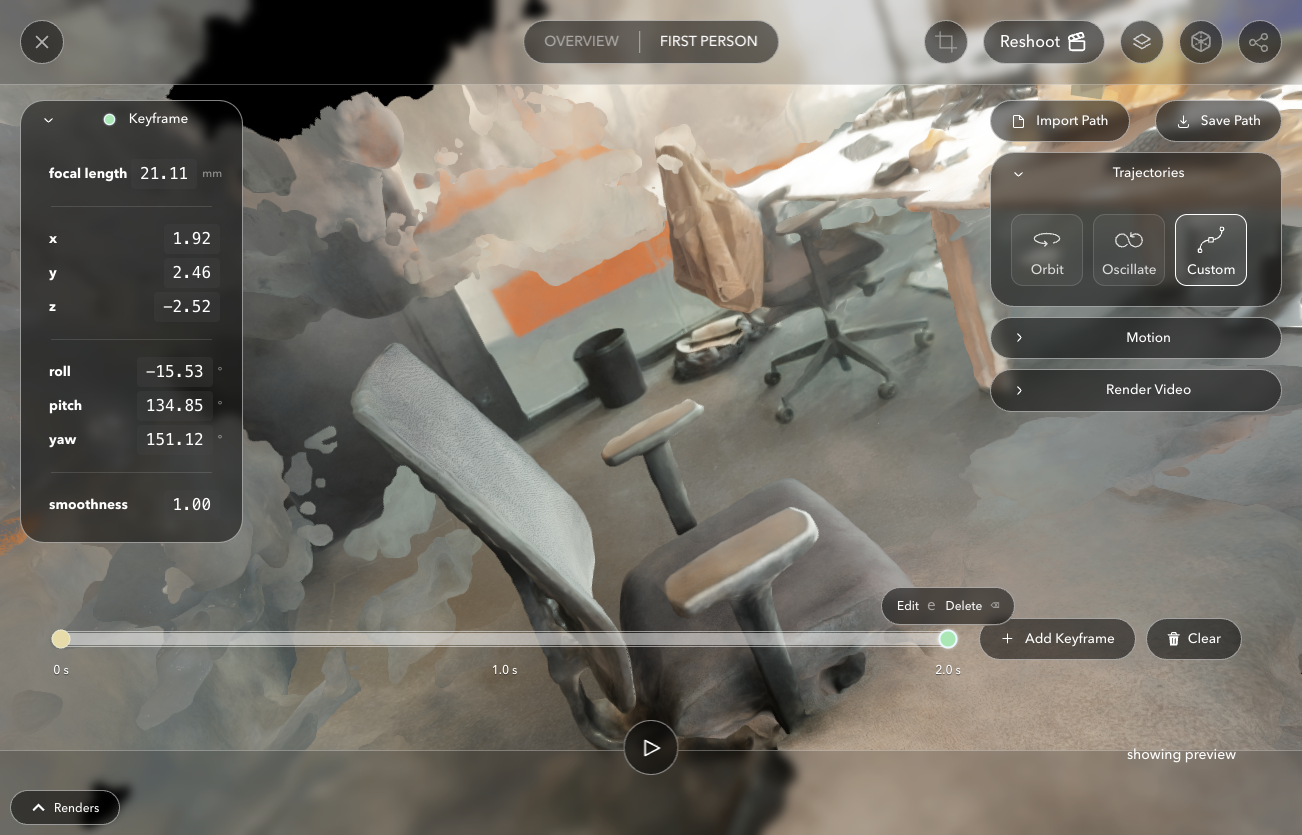
\includegraphics[width=\textwidth]{figures/related-luma.png}
  \caption{Luma AI Web Viewer in the camera path editor.}
  \label{fig:luma-viewer}
\end{figure}

\cleanparagraph{Export Capabilities}
Luma AI offers a variety of export formats for the generated scenes, allowing users to utilize these outputs in different applications or platforms, enhancing the utility of the captured NeRFs.
Additionally, they provide a social platform for the sharing and viewing of NeRFs, fostering a community of users around the technology.

\cleanparagraph{Limitations}
Despite its innovative approach, Luma AI's primary limitation lies in the lack of user control over the NeRF training process.
The automated system is designed to be user-friendly, yet it lacks the capacity to permit adjustments to the training parameters or the refinement of the final model.
This lack of control can result in suboptimal NeRF outputs for users who may require more precise or customized 3D representations.
Additionally, the proprietary nature of Luma AI may be a concern for users who prefer the flexibility and transparency offered by open-source solutions, as it limits the ability to understand and modify the underlying processes.

\section{Volinga Suite}

The Volinga Suite \cite{noauthor_volinga_nodate} aims to integrate Neural Radiance Fields into professional workflows.
It facilitates the adoption of NeRF by leveraging familiar platforms, thereby broadening the accessibility of NeRF to a wider range of users.

\cleanparagraph{Unreal Engine Integration}
Volinga's integration as a plugin for Unreal Engine \cite{noauthor_unreal_nodate} is a core feature that allows users to adopt NeRF seamlessly into existing pipelines \fref{fig:volinga-viewer}.
This integration is valuable for professionals already familiar with Unreal Engine, as it enables them to utilize advanced NeRF functionalities without additional training or significant adjustments to their current workflows.

\begin{figure}[h!]
  \centering
  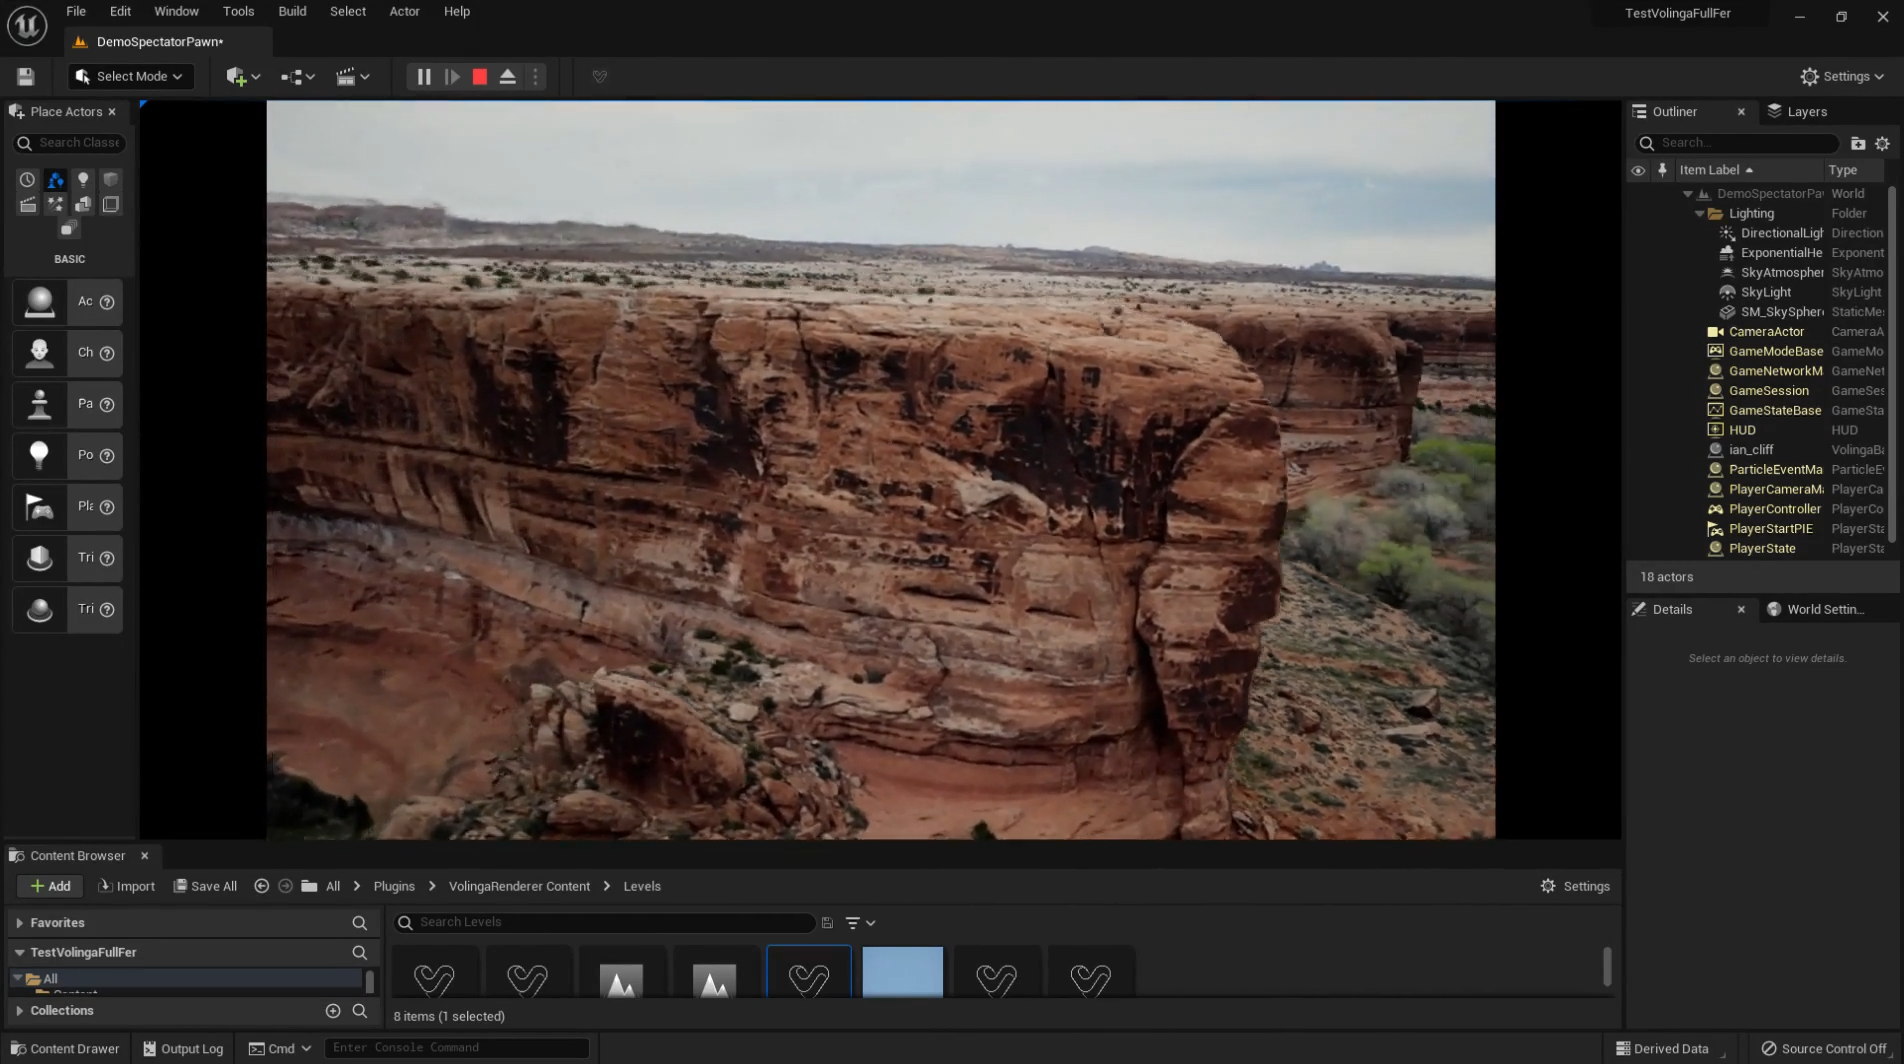
\includegraphics[width=\textwidth]{figures/related-volinga.png}
  \caption{Volinga Suite's integrated viewer in Unreal Engine \cite{noauthor_volinga_nodate}.}
  \label{fig:volinga-viewer}
\end{figure}

\cleanparagraph{Enhanced Control Over Training}
Volinga distinguishes itself from LumaAI by offering enhanced control over the NeRF training process.
Users have the ability to locally adjust numerous parameters, which enables precise tuning of the model's performance to meet specific project requirements.
This level of control is beneficial for projects where the quality of the NeRF output is critical.

\cleanparagraph{Local and Remote Training Capabilities}
The Volinga Creator component supports both local and remote training of NeRF models.
While remote training offers convenience and ease of access, local training provides advanced users with extensive configuration options and the ability to leverage powerful hardware, thereby maximizing the potential of NeRF technology under various usage scenarios.

\cleanparagraph{Limitations}
Volinga Suite's reliance on Unreal Engine for its integrated viewer may limit users who are unfamiliar with or do not wish to use this specific platform.
The web based viewer of Nerfstudio and Luma AI is more accessible in this regard.
Although Volinga is actively contributing to the open-source project Nerfstudio, its proprietary nature may also deter users or organizations that prefer open-source solutions.
